\documentclass[11pt,letterpaper]{article}
\usepackage[T1]{fontenc}
\usepackage[utf8]{inputenc}
\usepackage[margin=.86in,headheight=15pt]{geometry}
\usepackage{lmodern,mathpazo,amsmath,amssymb,amsthm,microtype}
\usepackage{booktabs,tabularx,array,longtable,enumitem,xcolor,tikz,fancyhdr,titlesec,needspace}
\usepackage{xurl,hyperref,listings,placeins}
\usetikzlibrary{arrows.meta,positioning,calc,fit,shapes.geometric}
\definecolor{ink}{HTML}{302045}
\definecolor{accent}{HTML}{7151A1}
\definecolor{gold}{HTML}{AC7F36}
\definecolor{pale}{HTML}{F5F2FA}
\definecolor{muted}{HTML}{665E70}
\hypersetup{colorlinks=true,linkcolor=accent,citecolor=accent,urlcolor=accent,pdftitle={Autonomous Enterprises: Activate. Evolve. Scale.},pdfauthor={Vincent Boucher},pdfsubject={SUCCESSOR Omega Harness: Constructing and Financing Reusable Productive Capability}}
\urlstyle{same}
\pagestyle{fancy}\fancyhf{}
\fancyhead[L]{\footnotesize\sffamily AUTONOMOUS ENTERPRISES}
\fancyhead[R]{\footnotesize\sffamily MONTREAL.AI / QUEBEC.AI}
\fancyfoot[C]{\thepage}\renewcommand{\headrulewidth}{.3pt}
\setlength{\parskip}{.26em}\setlength{\parindent}{1em}
\setlength{\emergencystretch}{3em}\renewcommand{\arraystretch}{1.13}
\setlist{nosep,leftmargin=1.4em}
\titleformat{\section}{\large\bfseries\color{ink}}{\thesection}{.65em}{}
\titleformat{\subsection}{\normalsize\bfseries\color{ink}}{\thesubsection}{.6em}{}
\titlespacing*{\section}{0pt}{1.15em}{.5em}
\titlespacing*{\subsection}{0pt}{.8em}{.35em}
\newcolumntype{Y}{>{\raggedright\arraybackslash}X}
\newcolumntype{P}[1]{>{\raggedright\arraybackslash}p{#1}}
\newcommand{\Om}{SUCCESSOR~$\Omega$}
\newcommand{\AGI}{\$AGIALPHA}
\newcommand{\insight}[1]{\begin{center}\setlength{\fboxsep}{9pt}\fcolorbox{accent}{pale}{\begin{minipage}{.93\linewidth}#1\end{minipage}}\end{center}}
\newtheorem{proposition}{Proposition}[section]
\newtheorem{theorem}[proposition]{Theorem}
\newtheorem{corollary}[proposition]{Corollary}
\lstset{basicstyle=\footnotesize\ttfamily,breaklines=true,columns=fullflexible,keepspaces=true,frame=single,rulecolor=\color{accent!35},showstringspaces=false}
\renewcommand{\topfraction}{.95}\renewcommand{\bottomfraction}{.9}\renewcommand{\textfraction}{.05}\renewcommand{\floatpagefraction}{.8}
\begin{document}
\thispagestyle{plain}
\begin{center}
{\small\sffamily\color{accent} MONTREAL.AI / QUEBEC.AI}\par
\vspace{.45em}

\begin{tikzpicture}[baseline=-.5ex]
\foreach \x/\y/\s in {0/0/.12,.33/.12/.055,.63/-.04/.08,.92/.16/.045,1.22/0/.12}{\node[star,star points=5,fill=gold,draw=none,minimum size=\s cm,inner sep=0pt] at (\x,\y) {};}
\draw[accent,line width=1.3pt] (1.6,0) circle (.13);\draw[accent,line width=1pt] (1.6,0) circle (.045);
\foreach \a in {0,45,...,315}{\draw[accent,line width=2pt] (1.6,0) ++(\a:.13)--++(\a:.055);}
\end{tikzpicture}\par
\vspace{.45em}
{\fontsize{25}{29}\selectfont\bfseries\color{ink} AUTONOMOUS ENTERPRISES}\par
\vspace{.38em}
{\fontsize{23}{27}\selectfont\bfseries\color{accent} ACTIVATE. EVOLVE. SCALE.}\par
\vspace{.7em}
{\large\bfseries \Om\ Harness}\par
\vspace{.2em}
{\large Constructing and Financing Reusable Productive Capability}\par
\vspace{.5em}
{\small\sffamily Powered by TRANSFORMATIONAL INTELLIGENCE $\infty$}\par
\vspace{.8em}
{\large Vincent Boucher}\par
MONTREAL.AI\quad\textbullet\quad QUEBEC.AI\par
Montr\'eal, Qu\'ebec, Canada\par
\vspace{.4em}
22 October 2026\quad\textbullet\quad Source-grounded research manuscript
\end{center}
\begin{abstract}
An enterprise should leave behind more than its delivery: it should improve the conditions under which the next useful enterprise can begin. We realize this principle as an operating path for the existing \Om\ Harness, separating off-chain capability construction from on-chain admission, commitments, financing and settlement. A concrete local companion constructs a bounded interval-measurement instrument and applies it to two distinct offerings: demand exposure reports and infrastructure capacity-violation certificates. The retained instrument removes repeated raw-overlap scans; each offering still receives a fresh semantic interpretation and independent output check. Independent setup, ordinary harness reuse and instrument reuse are compared, including construction and verification work, failed transfers and recovery. A strong conventional sweep implementation is credited explicitly; no new sweep algorithm or general recursive self-improvement is claimed. We map the owner-designated Ethereum five-contract deployment to exact source functions and preserve the separate USDC and \AGI\ Jobs routes. The deployed inventory, open harness candidate, replayed worker examples and new simulations are distinguished throughout. The contribution is an inspectable integration specification and runnable construction experiment, not autonomous incorporation, observed demand, investment performance or approved mainnet operation. Useful baselines can activate now; bounded improvement should accelerate their successors rather than prevent their launch.
\end{abstract}
\insight{\centering\textbf{Build what makes the next enterprise possible.}\par\smallskip
Activate available capability. Operate accountably. Retain what survives a fresh test.}
\begin{center}\small\textbf{FIND YOUR ALPHA. BUILD YOUR SUCCESSOR $\Omega$.}\par
\href{https://github.com/MontrealAI/AGI-Alpha-Agent-v0}{github.com/MontrealAI/AGI-Alpha-Agent-v0}
\end{center}
\clearpage

\section{The enterprise after the first result}
A planning team needs to know how much demand accumulated during several windows. An infrastructure operator needs the exact intervals during which simultaneous link loads exceed capacity. Both receive public, bounded integer interval records. The first needs an exposure report; the second needs an overload certificate. Repeatedly inspecting every raw interval for every requested window is an inherited production method, not part of either beneficiary's required outcome.

Construct a measurement instrument that converts interval endpoints into disjoint segments with a constant aggregate load on each segment. It can integrate exposure over a window or identify every capacity violation. The next offering inherits the qualified instrument, its input convention and its measurement evidence. It does not inherit the first customer's consent, the first workload's segmentation, or a decision that the new result is correct. A separate checker still evaluates the actual requested result. The instrument removes repeated interior-overlap scanning from production; it does not remove fresh input interpretation or acceptance.

This is deliberately recognizable engineering. Sweep lines, integration and typed interfaces already exist. A competent engineer can build the same instrument, and our strong conventional comparator does. The transformational move is to ask which alleged necessity belongs to the outcome and which belongs only to the inherited setup, then construct and test a replacement. The engineering contribution is an executable retained-capability boundary aligned to an existing enterprise harness and its real financing interfaces. The evidence does not support a new general optimization algorithm or superiority over expert engineering.

\insight{\textbf{What work do enterprises repeatedly perform because of an inherited setup, and what could we construct so future enterprises no longer need to perform it?}\par\smallskip
Keep the beneficiary's outcome, permitted actions and acceptance obligations fixed. Change the means.}

The ambition is a growing diversity of useful enterprises. It has no artificial ceiling of one organization or one offering. Yet a hundred renamed copies are not a hundred kinds of productive capability. Useful expansion changes a beneficiary, deliverable, instrument or production possibility and pays for the new interpretation, qualification and operating burden. The next enterprise is a test of inheritance, not a rhetorical multiplication of the first.

\subsection{Lineage and the actual contribution}
This manuscript continues the pinned 22 October \emph{Activate. Evolve. Scale.} paper, revision \texttt{3717c9ff\allowbreak{}b677751e\allowbreak{}1733a9ac\allowbreak{}7e010f5c\allowbreak{}877ef5d1}, and preserves the earlier \emph{Build the Means of Building}, \emph{Transformational Intelligence} and \emph{Invent the Economy} sources and URLs \cite{predecessor20261022,ti,economy}. Historical result identities remain historical; the new companion is a clearly identified reconstruction and extension, not independent reproduction of unavailable original raw records.

Three contributions are reviewable here. First, an outcome-preserving construction protocol makes a retained productive instrument useful across distinct offerings and exposes the cost of its inheritance. Second, an exact-source operating specification connects that path to the deployed Ascension suite without confusing commitments and votes with industrial truth. Third, a runnable local companion makes successful delivery, unsuccessful transfer, bounded resources, retained history and independent checking inspectable. The existing harness remains the platform. The companion supplies a small integration experiment and proposed adapter boundary rather than another control plane.

\section{Preserve the outcome; reconstruct the means}
Write a mission as $M=(I,O,A,P,B,D,R)$: allowed inputs, required output, acceptance predicate, permitted actions, resource ceiling, deadlines and applicable rights. These are operational obligations. A proposed representation change is eligible only when it preserves the relevant meaning of this tuple or makes an explicit, separately accepted change. A faster answer to a different question is not an improvement.

A retained capability is $K=(v,\mathcal{D},f,\mathcal{I},E,L)$: a version, supported domain, executable method, typed interface, evidence and provenance/lineage. Reuse requires a fresh compatibility check $\operatorname{applicable}(K,M)$ and a fresh decision under $A$. A schema can reject malformed records while accepting a semantically wrong unit, interval convention or objective. Hash equality can identify bytes while failing to establish their usefulness. Therefore interface compatibility, artifact identity and task acceptance are separate tests.

For the companion, intervals are half-open $[a,b)$ with integer endpoints and nonnegative integer loads. Let
\begin{equation}
 L(t)=\sum_i w_i\mathbf{1}_{[a_i,b_i)}(t).
\end{equation}
The instrument sorts endpoints and constructs a piecewise-constant representation of $L$. An exposure request returns $\int_u^v L(t)\,dt$ exactly in integer load-time units. A capacity request returns the maximal constant-load intervals where $L(t)>c$, with its declared reporting convention. These related mathematical operations serve different outcomes. They do not certify whether a supplied demand series is representative or whether an engineering capacity threshold is safe.

For every new dataset the instrument constructs its own segments. The inherited asset is executable machinery and its bounded qualification evidence, not cached answers or a claim that old measurements apply to new records. The independent checker uses raw intervals and a different defining calculation. Consequently the construction can reduce production work while verification remains expensive. The paper reports that cost rather than hiding it behind the word ``reusable.''

\subsection{A practical construction protocol}
Begin with an available implementation and deliver one bounded result. Observe a recurring obstacle in that actual procedure. State the counterfactual necessity: ``every new query scans all raw intervals.'' Propose a concrete alternative and list what still must happen: input validation, endpoint processing, current acceptance and accountable recovery. Execute both methods on matched requests. Retain the alternative only when its total burden is justified over the intended reuse horizon. Credit the conventional method whenever it provides the same result.

No mandatory discovery ritual precedes activation. A small report can run locally without a wallet, token purchase, funding campaign or recursive self-improvement system. More demanding models and adapters can join the same acceptance boundary when their execution is authorized and useful. A fixed library of supported work families is a sensible initial boundary; it is not unrestricted execution of invented code.

\section{One architecture, six responsibilities, continuous operation}
\textbf{AGI ALPHA organizes agents, tools, memory, work and validation. TRANSFORMATIONAL INTELLIGENCE $\infty$ constructs better conditions for discovery and production.} The six responsibilities remain the foundation. The \Om\ Harness turns them into a working path; it is neither a seventh stage nor a requirement for six model calls per task.

\begin{table}[htbp]\centering\small
\caption{Six responsibilities, each with a concrete obligation. A single tool call can serve several; some tasks require no model.}
\begin{tabularx}{\linewidth}{@{}P{2.65cm}YY@{}}\toprule
Responsibility & Work to perform & Boundary to preserve\\\midrule
OUT-LEARN & Find relevant evidence and uncertainty & Evidence relevance is not authority\\
OUT-THINK & Replace a restrictive representation & Preserve the outcome and constraints\\
OUT-DESIGN & Construct an enabling instrument or production boundary & Test an executable alternative\\
OUT-STRATEGISE & Identify necessary information and actions & Include qualification and recovery cost\\
OUT-EXECUTE & Deliver and check useful results & Retain valid progress and failed attempts\\
OUT-EVOLVE & Qualify means a successor can improve & New use needs fresh applicability and acceptance\\\bottomrule
\end{tabularx}
\end{table}

\textbf{ACTIVATE} an available capability around a worthwhile mission. \textbf{OPERATE} continuously: execute, validate, account, recover and retain. \textbf{EVOLVE} the means of creating and delivering useful offerings. \textbf{SCALE} the diverse offerings and shared capabilities that prove useful. OPERATE is the durable center even though the title emphasizes three verbs. Without execution, validation and recovery, a succession of plans produces no accepted work.

\begin{figure}[htbp]\centering
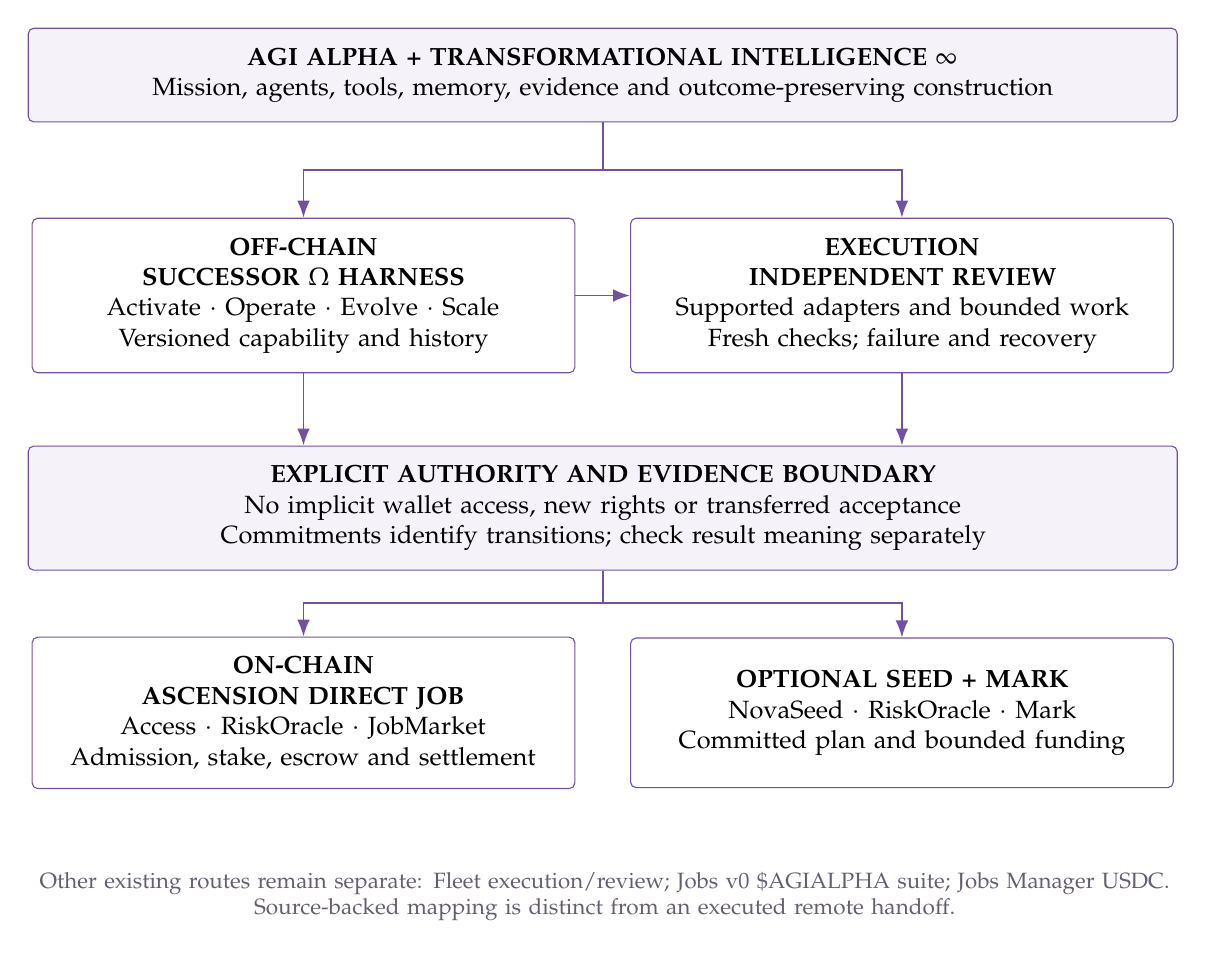
\begin{tikzpicture}[font=\small,>=Latex,
b/.style={draw=accent,rounded corners=2pt,align=center,inner sep=7pt},
arrow/.style={->,draw=accent,line width=.7pt}]
\node[b,fill=pale,text width=14.1cm] (a) at (0,0) {\textbf{AGI ALPHA + TRANSFORMATIONAL INTELLIGENCE $\infty$}\par Mission, agents, tools, memory, evidence and outcome-preserving construction};
\node[b,text width=6.4cm,minimum height=1.9cm] (h) at (-3.8,-2.8) {\textbf{OFF-CHAIN}\par\textbf{SUCCESSOR $\Omega$ HARNESS}\par Activate $\cdot$ Operate $\cdot$ Evolve $\cdot$ Scale\par Versioned capability and history};
\node[b,text width=6.4cm,minimum height=1.9cm] (e) at (3.8,-2.8) {\textbf{EXECUTION}\par\textbf{INDEPENDENT REVIEW}\par Supported adapters and bounded work\par Fresh checks; failure and recovery};
\draw[arrow] (a.south)--(0,-1.2)-|(h.north);
\draw[arrow] (a.south)--(0,-1.2)-|(e.north);
\draw[arrow] (h)--(e);
\node[b,fill=pale,text width=14.1cm] (i) at (0,-5.5) {\textbf{EXPLICIT AUTHORITY AND EVIDENCE BOUNDARY}\par No implicit wallet access, new rights or transferred acceptance\par Commitments identify transitions; check result meaning separately};
\draw[arrow] (h.south)--(h.south |- i.north);
\draw[arrow] (e.south)--(e.south |- i.north);
\node[b,text width=6.4cm,minimum height=1.9cm] (c) at (-3.8,-8.1) {\textbf{ON-CHAIN}\par\textbf{ASCENSION DIRECT JOB}\par Access $\cdot$ RiskOracle $\cdot$ JobMarket\par Admission, stake, escrow and settlement};
\node[b,text width=6.4cm,minimum height=1.9cm] (m) at (3.8,-8.1) {\textbf{OPTIONAL SEED + MARK}\par NovaSeed $\cdot$ RiskOracle $\cdot$ Mark\par Committed plan and bounded funding};
\draw[arrow] (i.south)--(0,-6.7)-|(c.north);
\draw[arrow] (i.south)--(0,-6.7)-|(m.north);
\node[align=center,text width=14.3cm,font=\footnotesize\color{muted},anchor=north] at (0,-10.0) {Other existing routes remain separate: Fleet execution/review; Jobs v0 \$AGIALPHA suite; Jobs Manager USDC.\par Source-backed mapping is distinct from an executed remote handoff.};
\end{tikzpicture}

\caption{Off-chain intelligence constructs and checks productive capability. On-chain components enforce their actual admission, escrow, decision and transfer rules. Evidence references connect the layers; neither layer by itself establishes customer demand or physical truth. The reference companion executes locally and simulates the marked transaction boundary.}
\label{fig:architecture}
\end{figure}

An enterprise record binds a mission to explicit resources, current authority, an executable version, review obligations and retained outcomes. The paper uses ``enterprise'' in that software-operating sense. Incorporation, legal personhood, ownership of intellectual property, customer consent and permission to use infrastructure require their own valid bases. Neither NFT parentage nor copied configuration supplies them.

\begin{figure}[htbp]\centering
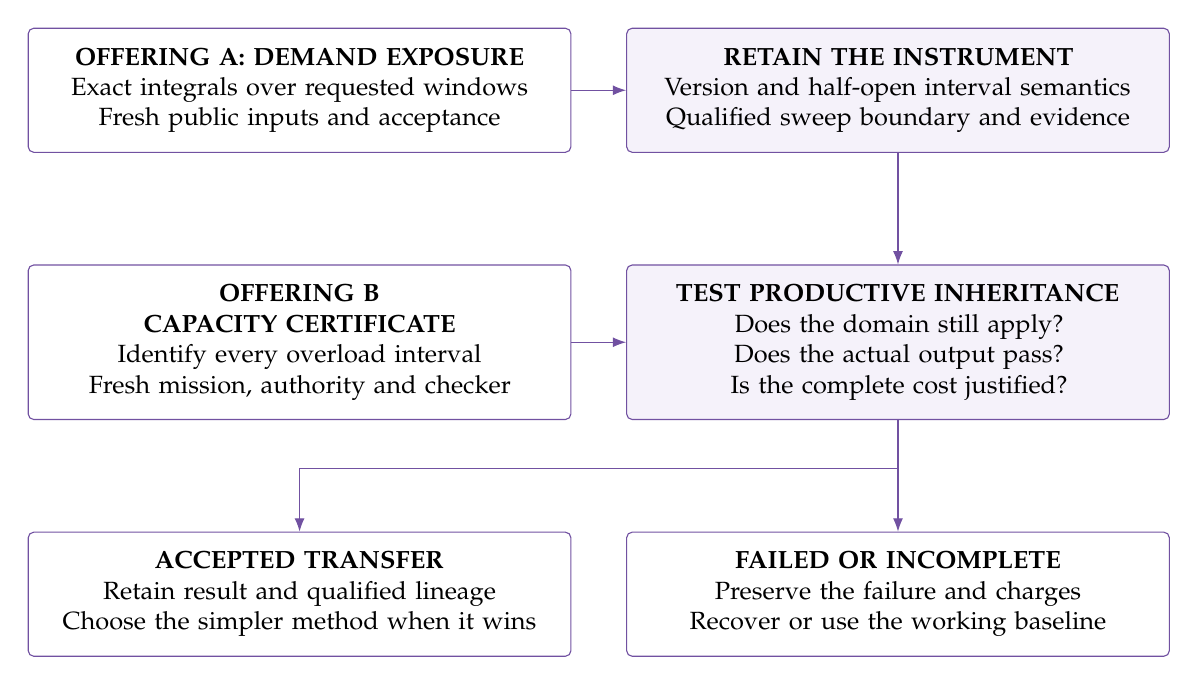
\begin{tikzpicture}[font=\small,>=Latex,
b/.style={draw=accent,rounded corners=2pt,align=center,inner sep=7pt},
arrow/.style={->,draw=accent}]
\node[b,text width=6.4cm,minimum height=1.25cm] (first) at (-3.8,0) {\textbf{OFFERING A: DEMAND EXPOSURE}\par Exact integrals over requested windows\par Fresh public inputs and acceptance};
\node[b,fill=pale,text width=6.4cm,minimum height=1.25cm] (retain) at (3.8,0) {\textbf{RETAIN THE INSTRUMENT}\par Version and half-open interval semantics\par Qualified sweep boundary and evidence};
\draw[arrow] (first)--(retain);
\node[b,text width=6.4cm,minimum height=1.6cm] (next) at (-3.8,-3.2) {\textbf{OFFERING B}\par\textbf{CAPACITY CERTIFICATE}\par Identify every overload interval\par Fresh mission, authority and checker};
\node[b,fill=pale,text width=6.4cm,minimum height=1.6cm] (eval) at (3.8,-3.2) {\textbf{TEST PRODUCTIVE INHERITANCE}\par Does the domain still apply?\par Does the actual output pass?\par Is the complete cost justified?};
\draw[arrow] (retain)--(eval);\draw[arrow] (next)--(eval);
\node[b,text width=6.4cm] (yes) at (-3.8,-6.4) {\textbf{ACCEPTED TRANSFER}\par Retain result and qualified lineage\par Choose the simpler method when it wins};
\node[b,text width=6.4cm] (no) at (3.8,-6.4) {\textbf{FAILED OR INCOMPLETE}\par Preserve the failure and charges\par Recover or use the working baseline};
\draw[arrow] (eval.south)--(3.8,-4.8)--(-3.8,-4.8)--(yes.north);
\draw[arrow] (eval.south)--(no.north);
\end{tikzpicture}

\caption{A successor inherits the instrument and applicable evidence, then qualifies the new meaning and result. A rejected transfer stays in the history. On-chain parentage can record lineage; only the off-chain qualification procedure tests productive inheritance.}
\label{fig:successor}
\end{figure}

\FloatBarrier
\section{The Ascension vision as an operating architecture}
``$\alpha$-AGI Ascension: Powered by \AGI'' becomes useful when each named role has an actual responsibility and evidence boundary. No new subsystem is needed merely to honor a name.

\begin{longtable}{@{}P{3.05cm}P{6.3cm}P{5.1cm}@{}}\toprule
Role & Mechanism in this architecture & What it does not establish\\\midrule\endhead
$\alpha$-AGI Insight & Develop testable hypotheses about unmet needs, beneficiaries and missions; retain disconfirming evidence & Beyond-human foresight, a trillion-dollar opportunity or observed demand\\
$\alpha$-AGI Nova-Seeds & ERC-721 lifecycle commits a capsule, immutable Merkle plan root, evidence and bounded job count; disclose plan material so consumers can verify commitments & Company equity, IP title, revenue rights or truth of disclosed claims\\
$\alpha$-AGI MARK & Supported curve-priced campaign contributions; phase-specific operations and committed-job routing & A general-purpose DEX, unrestricted treasury or guaranteed liquidity\\
$\alpha$-AGI Sovereign / Business & An admitted business identity operates a bounded mission with controlled resources, accepted outputs and accountable successors & Incorporation, legal sovereignty or autonomous legal agency\\
Large Scale $\alpha$-AGI Marketplace & Here: \texttt{AscensionJobMarket}, with funded jobs and source-defined bounded scoring, assignment, validation and settlement & Universally fastest/cheapest selection; the separate Jobs v0 suite\\
$\alpha$-AGI Agents & Eligible participants execute permitted off-chain work and submit result commitments and evidence URIs & A token holder's automatic eligibility or result correctness\\
$\alpha$-AGI Jobs & Define deliverables, funded rewards, deadlines and explicit acceptance evidence & Demand, profitability or universal work coverage\\
$\alpha$-AGI Architect & Propose, evaluate and version improvements to activation, instruments, execution and qualification & Unbounded self-modification or new spending authority\\
Validator Council / $\alpha$-AGI CLUB & Actual eligible, independent, staked reviewers make contract-supported decisions & Votes, incentives and tests being equivalent to proof of truth\\\bottomrule
\end{longtable}

A FusionPlan should be disclosed as a canonical set of committed job terms and its Merkle witnesses, together with the exact hashing/encoding convention consumed by the pinned contracts. The seed records commitments and metadata, not a complete business automatically executed by an NFT. A consumer verifies the disclosed plan against those commitments before relying on it. A hash alone supplies no disclosure, encryption quality, feasibility evidence or license.

The intended identities are \texttt{name.\allowbreak{}alpha.\allowbreak{}agi.\allowbreak{}eth}, \texttt{name.\allowbreak{}alpha.\allowbreak{}agent.\allowbreak{}agi.\allowbreak{}eth} and \texttt{name.\allowbreak{}alpha.\allowbreak{}club.\allowbreak{}agi.\allowbreak{}eth}. The access contract records an already-owned name under its configured role root; it does not mint a subname. Owner-issued admission, expiry, role registration and current ENS ownership are distinct conditions. Section~\ref{sec:contracts} details the pinned source rules and the missing root-observation evidence; intended spelling is not a live eligibility claim. The direction is a validator-gated constellation of enterprises. Achieved general intelligence, universal foresight and unconstrained autonomous sovereignty are not results of this manuscript.

\section{The deployed commitment and settlement boundary}
\label{sec:contracts}
The reference uses the owner-designated five-contract Ascension graph, rather than a newer-looking deployment or either separate Jobs system. We retrieved the deployment pointer, manifest and source on 22 October 2026. The manifest identifies Ethereum chain ID 1 and source revision \texttt{c0fc5217\allowbreak{}e364a39a\allowbreak{}4cd123d1\allowbreak{}7a8317c0\allowbreak{}6b80f820}; it reports five Etherscan exact matches and scoped authority observations at block 26,220,072, hash \texttt{0x8a3357d17\allowbreak{}a61a8f37\allowbreak{}c99dc836\allowbreak{}ac1176c6\allowbreak{}ee44b626\allowbreak{}1a81c418\allowbreak{}93527046\allowbreak{}c88a088}.\cite{manifest,deployment,ascensionsource} These are retained provider observations, not a fresh chain query in this study.

\begin{center}\small
\begin{tabular}{@{}ll@{}}
\toprule Component & Manifest address\\\midrule
AscensionAccess & \texttt{0x9eE41dF6d076Fa4F89b102b76DEf1c503a1e7C3A}\\
NovaSeed & \texttt{0x31BD0736DcD55DA2f9a2BB586C8a98695F86f19E}\\
AscensionRiskOracle & \texttt{0x198FC6EBee21c6A0B34E4d055AFD6D811AA6dE58}\\
AscensionJobMarket & \texttt{0xc1d3d7fb064C23c46C4EB20d24ab6EA650FF0ceE}\\
AscensionMark & \texttt{0x6D5323b2609E36fDc4dB3B2501B7BcF0E131033c}\\
\$\!AGIALPHA & \texttt{0xA61a3B3a130a9c20768EEBF97E21515A6046a1fA}\\
\bottomrule
\end{tabular}
\end{center}
All copied addresses were compared with the manifest or its token getters; token precision is 18 decimals. The dated record reports agent and validator minimum stakes of \(10^{19}\) base units, oracle quorum 2 and maximum risk 2,000 basis points. The minima and oracle parameters are constructor immutables in this source. It does not follow that a participant currently has sufficient stake, valid admission, live ENS ownership, approved allowance or an available reviewer.

\paragraph{Identity and authority.}
\texttt{AscensionAccess.\allowbreak{}Role} encodes Business \(=0\), Agent \(=1\), Validator \(=2\). Its constructor derives the roots \texttt{alpha.\allowbreak{}agi.\allowbreak{}eth}, \texttt{alpha.\allowbreak{}agent.\allowbreak{}agi.\allowbreak{}eth} and \texttt{alpha.\allowbreak{}club.\allowbreak{}agi.\allowbreak{}eth}. Registering \texttt{label} therefore records \texttt{label.\allowbreak{}alpha.\allowbreak{}agi.\allowbreak{}eth}, \texttt{label.\allowbreak{}alpha.\allowbreak{}agent.\allowbreak{}agi.\allowbreak{}eth} or \texttt{label.\allowbreak{}alpha.\allowbreak{}club.\allowbreak{}agi.\allowbreak{}eth}. Labels contain 1--63 bytes: lowercase ASCII letters, digits and interior hyphens only. The registration call checks the current ENS owner, or the current unexpired NameWrapper owner when the registry points to the configured wrapper. It does not use a resolver address as ownership.

Registration and admission are separate. Only the Access owner can call \texttt{setAdmission}; a positive admission requires nonzero evidence and expiry strictly after now and at most 365 days ahead. Setting expiry to zero revokes it. \texttt{eligible(\allowbreak{}account,\allowbreak{}role)} requires both unexpired admission and current ownership of that account's recorded role name. The source fixes the root construction, but this study did not read current root getters or any named participant from mainnet. It consequently asserts no live eligible identity. A software business identity is neither incorporation nor legal personhood.

\paragraph{Configuration is not operation.}
The Oracle's \texttt{bindMarketplace(\allowbreak{}address)} and JobMarket's \texttt{bindMark(\allowbreak{}address)} are owner-only, one-time bindings with reciprocal graph checks. Their finalized transactions are reported at blocks 26,219,975 and 26,220,058. Ownable2Step ownership is transferable storage, not immutable governance. The manifest records the governor \texttt{0xd76AD27a1Bcf8652e7e46BE603FA742FD1c10A99} for Access, Oracle and JobMarket, with zero pending owners at the authority block. NovaSeed and MARK have no owner administrator in this source. There is no global Solidity pause or unpause function. The manifest's \texttt{activationAllowed=false} and \texttt{readyForPublicFunding=false} are off-chain readiness declarations; they do not stop a Solidity call. The published pointer still states that activation and public funding are not approved. Independent security review, external authority inventory, exact-source real-dependency fork evidence and participant commissioning remain separate requirements.

\subsection{Callable feature map}
Tables~\ref{tab:accessmap}--\ref{tab:markmap} map the claims to the exact named callable, actor, transition, event and representative reverting condition. Full typed argument lists and ABI provenance are included in the companion's call map. Events record contract decisions; they do not certify external semantics.

\begin{table}[htbp]\centering\small
\caption{Identity, plan and risk calls at the pinned source.}\label{tab:accessmap}
\begin{tabularx}{\linewidth}{@{}P{.22\linewidth}YP{.24\linewidth}@{}}
\toprule Callable / actor & Prerequisite and state transition & Event / representative failure\\\midrule
\texttt{register(\allowbreak{}role,\allowbreak{}label)} / name owner & Canonical label and live ENS ownership; stores the role node. & \texttt{Registered}; noncanonical label or ownership absent.\\
\texttt{setAdmission(\allowbreak{}account,\allowbreak{}evidence,\allowbreak{}until)} / Access owner & Valid account and bounded expiry; writes or revokes admission. & \texttt{AdmissionSet}; invalid admission or non-owner.\\
\texttt{seal(\allowbreak{}.\allowbreak{}.\allowbreak{}.\allowbreak{})} / eligible business & Nonzero commitments, 1--128 jobs, 1--512-byte URI; optional parent currently owned by caller. Mints NFT and immutable genome. & \texttt{SeedSealed}; empty commitment or parent ownership.\\
\texttt{deposit(\allowbreak{}amount)}, \texttt{withdraw(\allowbreak{}amount)} / validator & Deposit: eligible validator and exact token receipt. Withdrawal: positive balance and now strictly beyond \texttt{lockedUntil}. & \texttt{StakeChanged}; validator identity or locked stake.\\
\texttt{setJobAvailability(\allowbreak{}business,\allowbreak{}until,\allowbreak{}capacity)} / validator account & Nonzero business; expiry zero or within 120 days; capacity at most 128. Records caller-offered availability for a business and shared caller capacity. & \texttt{JobAvailability}; availability bounds.\\
\texttt{openReview(\allowbreak{}id)} / eligible seed owner & Prior round strictly expired. Starts a seven-day round tied to the present owner. & \texttt{ReviewOpened}; seed owner or review still active.\\
\texttt{attest(\allowbreak{}id,\allowbreak{}riskBps,\allowbreak{}policyApproved,\allowbreak{}evidenceHash)} / staked validator & Current review/owner; validator differs from owner and original creator; one vote, nonzero evidence. Locks stake until round expiry; increments yes or no. & \texttt{RiskAttested}; duplicate, decided, expired or non-independent review.\\
\texttt{green(\allowbreak{}id)} / any reader & Requires quorum yes, unexpired round, same owner, eligible business and still-qualified supporting validators. & View only; returns false when a condition lapses.\\
\bottomrule
\end{tabularx}
\end{table}

\begin{table}[htbp]\centering\small
\caption{Direct and MARK-originated job calls.}\label{tab:jobmap}
\begin{tabularx}{\linewidth}{@{}P{.22\linewidth}YP{.24\linewidth}@{}}
\toprule Callable / actor & Prerequisite and state transition & Event / representative failure\\\midrule
\texttt{deposit(\allowbreak{}amount)}, \texttt{withdraw(\allowbreak{}amount)} / agent & Deposit requires eligible Agent and exact receipt; withdrawal cannot consume locked collateral. & \texttt{StakeChanged}; agent identity or locked stake.\\
\texttt{post(\allowbreak{}spec,\allowbreak{}auctionSeconds,\allowbreak{}validators)} / eligible business & Bounds and three independent reviewers; reserves capacity and escrows bounty from caller. Creates Auction. & \texttt{JobPosted}; job bounds, committee conflict or unavailable capacity.\\
\texttt{postFromSeed(\allowbreak{}business,\allowbreak{}.\allowbreak{}.\allowbreak{}.\allowbreak{})} / bound MARK only & Same job checks; MARK is token payer and refund client, nominated business is enterprise principal. & \texttt{JobPosted}; MARK only.\\
\texttt{bid(\allowbreak{}id,\allowbreak{}price,\allowbreak{}duration)} / eligible agent & Open auction, no role conflict, at most 32 distinct bidders; locks the job bond. & \texttt{BidPlaced}; invalid bounds, duplicate or insufficient free stake.\\
\texttt{award(\allowbreak{}id)} / any caller & Auction ended. Chooses lowest eligible score fitting remaining execution horizon; unlocks losers. No winner produces Refunded. & \texttt{Assigned} or \texttt{Closed}; auction not ended.\\
\texttt{submit(\allowbreak{}id,\allowbreak{}resultHash,\allowbreak{}resultURI)} / assigned worker & Assigned, eligible Agent and now at or before due; nonzero commitment and bounded URI. Creates Submitted. & \texttt{Delivered}; not deliverable or result required.\\
\texttt{validate(\allowbreak{}id,\allowbreak{}resultHash,\allowbreak{}approved,\allowbreak{}evidence)} / selected validator & Submitted and now at or before review end; same artifact, current stake/eligibility, one vote. Second yes pays; second no fails with slashing. & \texttt{Validated}, \texttt{Payout}, \texttt{Closed}; artifact, duplicate or eligibility failure.\\
\texttt{timeout(\allowbreak{}id)} / any caller & Assigned past due: slash and Failed. Submitted past review end: Refunded without slashing. & \texttt{Closed}; delivery/review still open.\\
\texttt{claimRefund(\allowbreak{}id)} / recorded client only & Terminal job, not previously claimed. Transfers accrued refund once. & \texttt{RefundClaimed}; refund unavailable.\\
\bottomrule
\end{tabularx}
\end{table}

\subsection{The minimal direct-job journey}
Start without a wallet for local mission design, evaluation and unfunded computation. Add the chain only for a separately authorized funded commitment. The exact source uses
\[
\begin{aligned}\texttt{Spec}=(&\texttt{string goal, string successMetric, uint96 bounty},\\ &\texttt{uint32 duration, uint16 priceWeight}).\end{aligned}
\]
All monetary fields are integer token base units and all durations are seconds. The reference order is as follows.

\begin{enumerate}
\item Each role holder calls Access \texttt{register(\allowbreak{}role,\allowbreak{}label)} for its owned name. The Access owner separately supplies a valid \texttt{setAdmission(\allowbreak{}account,\allowbreak{}evidence,\allowbreak{}until)}. An already admitted holder need not repeat a valid registration.
\item Agents approve the \emph{JobMarket} as token spender and call its \texttt{deposit(\allowbreak{}uint256)}. Each validator approves the \emph{Oracle}, calls its \texttt{deposit(\allowbreak{}uint256)}, and records \texttt{setJobAvailability(\allowbreak{}business,\allowbreak{}until,\allowbreak{}capacity)} covering the entire job horizon.
\item The eligible business approves the \emph{JobMarket} for the bounty and calls \texttt{post(\allowbreak{}Spec,\allowbreak{}uint32,\allowbreak{}address[\allowbreak{}3])}. Goal and success metric each contain 1--512 bytes; bounty is at least 100 base units; duration is positive and at most 90 days; auction duration is positive and at most seven days; price weight is at most 10,000. The job bond is \(\max(\lfloor B/10\rfloor,m)\), with bounty \(B\) and minimum \(m\). Three distinct current Oracle validators must differ from the business and token-paying caller.
\item Before auction end, each agent calls \texttt{bid(\allowbreak{}uint256,\allowbreak{}uint96,\allowbreak{}uint32)} with price from 100 through \(B\), positive duration no greater than the specification, and enough free deposited stake to lock the bond. A committee member cannot bid on that job.
\item At or after auction end, any caller invokes \texttt{award(\allowbreak{}uint256)}. The winner is the lowest implemented score among still-eligible bids that fit the remaining execution horizon; this is a bounded auction, not universal optimal agent selection. Ties use lower price, shorter duration and then lower numerical address. Every losing bond is unlocked. With no admissible winner, the full bounty becomes refundable.
\item The assigned worker performs the supported off-chain work, retains exact bytes and checker results, and calls \texttt{submit(\allowbreak{}uint256,\allowbreak{}bytes32,\allowbreak{}string)} by its due time. The contract stores the commitment and emits the URI. Each selected validator independently obtains those bytes, checks their commitment and acceptance evidence, then calls \texttt{validate(\allowbreak{}uint256,\allowbreak{}bytes32,\allowbreak{}bool,\allowbreak{}bytes32)}.
\item Two approvals trigger payment inside the second successful validation transaction. The harness independently verifies the terminal state and actual artifact acceptance before retaining a qualified capability. The client calls \texttt{claimRefund(\allowbreak{}uint256)} for unused bounty. A successor receives qualified artifacts and evidence, while obtaining its own authority, funding and task-specific acceptance.
\end{enumerate}

For bid price \(p\), promised duration \(d\), bounty \(B\), maximum duration \(D\), price weight \(w\), and reputation snapshot \(r\), the exact integer score is
\[
c=\left\lfloor\frac{pw10^6}{B}\right\rfloor,\quad
t=\left\lfloor\frac{d(10000-w)10^6}{D}\right\rfloor,\quad
s=\left\lfloor\frac{(c+t)10000}{10000+\min(r,10000)}\right\rfloor .
\]
Reputation here is the JobMarket's own bounded accepted-job counter, captured at bid time. It is not a general claim about an agent. Successful settlement increments it by one, capped at 10,000; a slashed failure decreases a positive value by one.

\paragraph{Quorum, arithmetic and recovery.}
The committee has three validators. Two approvals settle immediately; two rejections fail with slashing. Earlier approving or rejecting voters are rechecked for current Oracle eligibility when their decisive branch executes. Worker eligibility is checked at submission; the payout branch does not recheck worker or business eligibility. If \(p\) is the agreed price, each approving validator's gross payout is
\[
v=\left\lfloor\frac{\left\lfloor500p/10000\right\rfloor}{2}\right\rfloor,\qquad
g_{\rm worker}=p-2v .
\]
Thus the nominal 95/5 split has rounding dust assigned to the worker. Every gross payout \(g\) burns \(\lfloor g/100\rfloor\) and transfers the remainder. With \(p=100\) tokens, the worker receives 94.05 tokens, each of the two approving validators receives 2.475, and one token is burned. Only the two approving validators are paid. The difference \(B-p\) is a separate client refund, not a worker payout.

A missed worker due time permits anyone to call \texttt{timeout}: the bond is removed from agent stake, one percent of it is burned with integer rounding, and its remainder is added to the client's full-bounty refund. A two-rejection decision follows the same slash branch. The slash emits a \texttt{Payout} event for the client while crediting the refund; actual transfer occurs later in \texttt{claimRefund}. Missing reviewer quorum after submission instead returns the bounty and unlocks worker collateral without slashing: missing quorum is not proof of defective work. There is no general business cancellation call. Award, timeout and refund collection require calls; passing a deadline alone does not execute them. Terminal jobs release reviewer active-job capacity, but do not shorten the Oracle's previously established stake lock deadline.

\subsection{Optional NovaSeed and MARK financing}
A FusionPlan discloses a bounded set of committed job specifications and proofs against an immutable Merkle root. Its contract commitment does not itself publish the plan contents: collaborators must retain and disclose the exact job specifications, indexes, hashing convention and Merkle proofs. JobMarket \texttt{hashSpec(\allowbreak{}index,\allowbreak{}spec)} computes a double-keccak leaf from ABI-encoded index, hashed goal and metric, bounty, duration and price weight. MARK verifies the actual plan index; the job itself stores \texttt{hashSpec(\allowbreak{}0,\allowbreak{}spec)}, so a nonzero plan leaf and the stored job hash must not be equated. MARK verifies the proof using OpenZeppelin's sorted-pair Merkle convention. A seed's NFT records the capsule, plan and evidence commitments, original creator, bounded job count and optional parent. It does not automatically transfer equity, intellectual property, revenue rights or proven capability inheritance.

\begin{table}[htbp]\centering\small
\caption{Optional campaign calls; MARK lots are internal campaign accounting.}\label{tab:markmap}
\begin{tabularx}{\linewidth}{@{}P{.22\linewidth}YP{.24\linewidth}@{}}
\toprule Callable / actor & Prerequisite and state transition & Event / representative failure\\\midrule
\texttt{open(\allowbreak{}id,\allowbreak{}base,\allowbreak{}slope,\allowbreak{}maxLots,\allowbreak{}target,\allowbreak{}fundingEnd,\allowbreak{}duration)} / green seed owner & No prior campaign; bounded reachable target and horizon. Records business and ENS node; creates Funding. & \texttt{MarketOpened}; green owner, bounds or unreachable target.\\
\texttt{buy(\allowbreak{}id,\allowbreak{}count,\allowbreak{}maxCost)} / admitted buyer & Before funding end; green decision and unchanged seed owner; bounded lot count and quoted cost. Receives tokens; increases lots and reserve. & \texttt{Traded}; admission gate, lot bound or slippage.\\
\texttt{sell(\allowbreak{}id,\allowbreak{}count,\allowbreak{}minReturn)} / lot holder & Funding phase and sufficient lots. Returns reverse-curve value; no admission or green recheck and no funding-deadline check. & \texttt{Traded}; not redeemable or slippage.\\
\texttt{transferLots(\allowbreak{}id,\allowbreak{}to,\allowbreak{}count)} / admitted holder & Funding before deadline; green and unchanged owner; both parties admitted. Moves internal lots without payment. & \texttt{LotsTransferred}; funding/admission gate.\\
\texttt{bloom(\allowbreak{}id)} / recorded business & Funding before deadline, reserve reaches target, current green owner and still-owned recorded ENS node. Creates Bloomed. & \texttt{Bloomed}; not funded or business authority.\\
\texttt{route(\allowbreak{}id,\allowbreak{}index,\allowbreak{}spec,\allowbreak{}proof,\allowbreak{}auctionSeconds,\allowbreak{}validators)} / recorded business & Bloomed, same seed owner, green, node ownership, horizon, valid unused plan leaf and reserve. Exact bounty allowance to Jobs, call \texttt{postFromSeed}, then clear allowance. & \texttt{MissionRouted}; authority, plan proof, budget or job failure.\\
\texttt{collect(\allowbreak{}jobId)} / any caller & Routed terminal job not collected. Pulls job refund into reserve and reduces active count. & \texttt{MissionCollected}; not collectible.\\
\texttt{close(\allowbreak{}id)} / any caller & Funding at/after funding end; or Bloomed with no active jobs and all plan jobs posted or execution end strictly passed. Creates Closed. & \texttt{CampaignClosed}; funding/missions still open.\\
\texttt{reclaim(\allowbreak{}id)} / lot holder & Closed and positive holdings; consumes holder's lots and returns proportional unused reserve. & \texttt{CapitalReturned}; no capital claim.\\
\bottomrule
\end{tabularx}
\end{table}

The typed seed call is \texttt{seal(\allowbreak{}bytes32 capsuleHash,\allowbreak{}bytes32 planRoot,\allowbreak{}uint32 jobs,\allowbreak{}string metadataURI,\allowbreak{}uint256 parent,\allowbreak{}bytes32 evidenceHash)}. For a first seed, parent is zero; otherwise the caller must own the parent at sealing. The eligible owner then calls Oracle \texttt{openReview(\allowbreak{}uint256)}. Eligible staked validators, independent of both current seed owner and original creator, call \texttt{attest(\allowbreak{}uint256,\allowbreak{}uint16,\allowbreak{}bool,\allowbreak{}bytes32)}. A yes requires policy approval and reported risk no greater than the configured threshold. A decisive no quorum prevents further votes, but this is a risk-policy round, not job-output acceptance.

A green owner may next call MARK \texttt{open(\allowbreak{}uint256,\allowbreak{}uint96,\allowbreak{}uint96,\allowbreak{}uint32,\allowbreak{}uint96,\allowbreak{}uint64,\allowbreak{}uint32)}. Base is positive; slope may be zero; maximum supply is 1--1,000,000 lots; target is positive and no greater than the full curve quote; funding ends within 30 days; execution duration is greater than the three-day review window and at most 90 days. For supply \(s\), count \(n\), base \(b\) and slope \(a\), the curve quote is
\[
Q(s,n)=nb+\left\lfloor an(2s+n-1)/2\right\rfloor
\]
for \(n>0\), with \(Q(s,0)=0\). Buyers approve \emph{MARK}, then \texttt{buy(\allowbreak{}uint256,\allowbreak{}uint32,\allowbreak{}uint256)} caps cost; \texttt{sell(\allowbreak{}uint256,\allowbreak{}uint32,\allowbreak{}uint256)} floors return using \(Q(s-n,n)\). These are campaign lots, not a newly issued ERC-20, an unrestricted DEX or a guaranteed liquid secondary market.

When reserve reaches target, the recorded business calls \texttt{bloom}. The business can then \texttt{route(\allowbreak{}uint256,\allowbreak{}uint32,\allowbreak{}Spec,\allowbreak{}bytes32[\allowbreak{}],\allowbreak{}uint32,\allowbreak{}address[\allowbreak{}3])} only for a committed, unused plan index with sufficient reserve and time for auction, execution and review. MARK, not the business wallet, is the job client and allowance source. Its exact bounty approval is cleared after the call. The reserve cannot be freely withdrawn as an enterprise treasury.

Oracle green lasts only through its seven-day round and is sensitive to owner, admission and supporting-validator changes. A 30-day funding window or longer campaign does not extend that approval. A fresh round may be needed before later buys, bloom or routing; a new round cannot start until the prior round is strictly expired. Already posted jobs have their own independent review lifecycle. On closure, \texttt{reclaim} returns \(\lfloor R h/S\rfloor\) for remaining reserve \(R\), holder lots \(h\), and remaining supply \(S\), then removes both the paid reserve and consumed lots. The final claimant receives the final residual. This is unused-capital recovery, not promised profit or revenue distribution.

\paragraph{Token utility and its cost.}
Agent deposits secure locked performance collateral; validator deposits support eligibility and timed review locks; funded bounty escrow supports agreed delivery and review payments; MARK contributions fund committed jobs. Deposits, ordinary transfers, curve purchases/sales, reserve recovery and bounty refunds are not all subject to the payout burn. \texttt{AscensionToken} checks exact transfer receipts and recipients, 18-decimal precision and actual supply destruction for its burn calls. A token holder is not thereby an admitted business, eligible worker, reviewer or payout recipient. Against a competent centralized system, this route adds gas, capital lockup, reviewer cost, latency and explicit recovery calls. Its potential benefit is inspectable commitments and rule-bound settlement among separately admitted participants; customer demand and commercial advantage remain to be demonstrated.

\paragraph{ABI and execution evidence boundary.}
We inspected the pinned Solidity declarations and a pinned historical compiled ABI archive, and supplied a source-compatible call ABI with an explicit provenance record. The historical wallet profile embeds 11 October addresses and must not be used to select this deployment. This study did not retrieve bytes authenticating the 18 October explorer ABI hashes or execute these calls on mainnet. The runnable companion is a labeled local transition model with its own checker, not a claim of Solidity conformance, a fork reproduction or a transaction-ready client. A future authorized operator must authenticate the complete deployed ABI, live graph and participant state before signing.


\FloatBarrier
\section{Implementation: one harness, explicit route boundaries}\label{sec:harness}

The reference extends AGI ALPHA's maintained operating path rather than introducing another enterprise service. The inspected \texttt{successor-\allowbreak{}harness} facade is PR~4863 at
\texttt{c455ad4c\allowbreak{}e109c86d\allowbreak{}f2fef09d\allowbreak{}19674810\allowbreak{}290b5185}. On 22~October~2026 the refreshed PR record was \emph{open, not merged}, with that exact head. It therefore supplies candidate source, not released or deployed functionality.\footnote{\url{https://github.com/MontrealAI/AGI-Alpha-Agent-v0/pull/4863}}
The retrieved workflow-runs and combined-status responses contained no entries; these responses do not establish hosted qualification or publication. The PR's report of 34 passing harness/workbench tests remains an external author report in this paper; we inspected the tests but did not rerun the complete Python facade environment.

\subsection{What the candidate actually retains and executes}

\texttt{enterprise.\allowbreak{}py} accepts exactly five top-level fields:
\texttt{schema}, \texttt{enterprise\_\allowbreak{}id}, \texttt{name}, \texttt{work}, and
\texttt{parent}. The schema is \texttt{successor-\allowbreak{}enterprise/\allowbreak{}v1}; an enterprise ID is a canonical UUID. The work request is validated through the existing workbench before registration. The immutable configuration and work record are retained in the existing SQLite journal, whose entries form a hash chain signed by its local Ed25519 identity. This supplies source attribution and tamper detection relative to retained keys/checkpoints; it is not independent organizational review or proof that an operator never rewrote its own history.

\begin{table}[htbp]
\centering\small
\begin{tabularx}{\linewidth}{@{}p{.21\linewidth}XX@{}}
\toprule
Actual entry point & Result & Boundary preserved\\
\midrule
\texttt{new}, \texttt{validate} & Editable, inert configuration for a maintained family. & No journal or permission is created by template preparation.\\
\texttt{activate} & Configuration and planned work run registered; repeated identical activation is idempotent. & An ID cannot bind changed configuration; an exact accepted parent is checked again in the registration transaction.\\
\texttt{operate} & Fixed worker runs; completed output awaits result-bound local review. & Completed terminal results are retained; retries do not silently erase prior attempts.\\
\texttt{review}, \texttt{export} & Exact result digest accepted/rejected; artifacts and signed local receipt exported. & Review records the local operator and \texttt{independent=False}. A recipient needs separately trusted source keys.\\
\texttt{derive} & New UUID and editable work template with exact parent configuration/result digests. & Child begins planned, without its parent's result, acceptance, authority or settlement.\\
\texttt{handoff} & Existing Studio request bound to enterprise work and a verified plan index. & Validation is not execution, profile installation, a grant, or funding.\\
\bottomrule
\end{tabularx}
\caption{Pinned candidate behavior, established by source inspection. Full paths and blob identities are retained in the companion evidence.}
\end{table}

The five maintained families are reliability, performance, documentation, public-data and numerical. \texttt{workbench.\allowbreak{}invoke} invokes the packaged Node worker with bounded JSON, a scrubbed environment and cancellation checks. It cannot select a caller-supplied executable. The local path has three attempts, a declared 60\,000\,ms per-attempt budget, and a 65-second outer watchdog; these are distinct implementation bounds. Compute price and human-review cost are explicitly unknown. The local states include planned, running, review, accepted, rejected, interrupted, paused, stopped and retired. Resume is explicit for interrupted/paused pure work; stop and retirement are terminal.

We executed the exact pinned worker directly on its included numerical and public-data examples, then ran its inspection operation. The numerical output reports the exact integral of $x^2$ over $[0,3]$ as $9$, Simpson's result as $9$, and the retained trapezoid error as $1/32$, which fails the declared $10^{-6}$ tolerance. The public-data report retains five rows and group totals 60, 155 and 80, summing to 295. These are local fixed-worker executions, not runs of the full enterprise facade, independently commissioned services or on-chain settlements. Their raw requests, results and inspection records are supplied separately. They establish a working bounded baseline while the new construction is evaluated.

The companion also exercises a concrete integration: \texttt{harness\_\allowbreak{}adapter.\allowbreak{}py} verifies the new instrument's retained exposure result and converts all 80 window/value pairs into the existing public-data CSV interface. Each row retains its unique window index and bounds; units explicitly warn that summing overlapping windows counts exposure repeatedly. The adapter invokes the pinned worker's actual \texttt{plan}, \texttt{run} and \texttt{inspect} operations. A separate Python check compares every group and the delivered CSV/JSON artifacts against the interval result. It also emits a valid-shaped \texttt{successor-\allowbreak{}enterprise/\allowbreak{}v1} configuration for later activation. The worker formats this exact report; the new instrument executes in the Python companion. Neither the full enterprise facade nor a native signed journal was activated by this integration.

\subsection{Studio and the three economic routes}

The actual handoff schema is \texttt{agialpha.\allowbreak{}ascension.\allowbreak{}studio-\allowbreak{}work.\allowbreak{}v1}, containing exactly
\texttt{schema}, \texttt{project\_\allowbreak{}id}, \texttt{cycle\_\allowbreak{}id}, \texttt{plan},
\texttt{plan\_\allowbreak{}index} and \texttt{work\_\allowbreak{}spec}. Plan verification and a valid index bind the selected work; they do not establish remote capacity. Existing Studio functions
\texttt{prepare\_\allowbreak{}work}, \texttt{seal\_\allowbreak{}work}, \texttt{bind\_\allowbreak{}work},
\texttt{execute\_\allowbreak{}work}, \texttt{accept\_\allowbreak{}work} and \texttt{settle\_\allowbreak{}work}
own their respective boundaries. Execution checks the installed environment and exact controller-signed authorization. The read-only Ascension adapter binds canonical posting and assignment observations, commits delivered bytes, and reconciles contract facts. Local acceptance and the market's validator decision are separate records.

\begin{table}[htbp]
\centering\small
\begin{tabularx}{\linewidth}{@{}p{.20\linewidth}XX@{}}
\toprule
Route / source & Inspected interface & What remains separate\\
\midrule
Alpha / Ascension & Studio request and \texttt{MarketReader}; \texttt{bind\_\allowbreak{}assignment}, \texttt{bind\_\allowbreak{}delivery}, \texttt{import\_\allowbreak{}settlement}. & The designated five-contract graph, AGIALPHA in 18 decimals, installed trust and explicit grants.\\
Fleet Linux & \texttt{SuccessorController.\allowbreak{}prepare}, \texttt{execute}, \texttt{result}, \texttt{stop}; installed Controller $\rightarrow$ Studio $\rightarrow$ Companion $\rightarrow$ ComputeWorker. & Current runtime health, exact task, session-bound confirmation and worker/reviewer control; an internal checker is not independent control.\\
Jobs v0 & \texttt{importAlphaProject}, \texttt{runProjectTransfer}, \texttt{inspectProjectTransfer}, \texttt{verifyProjectReceipt}. & A distinct AGIALPHA \emph{JobRegistry} route; unfunded drafts and receipt checks do not grant authority or reconcile payouts.\\
Jobs Manager & \texttt{prepareImprovement}; native employer-model/console interfaces and \texttt{compileComputerWork}. & A separate six-decimal USDC draft, current admission, runtime context and authorized console action.\\
\bottomrule
\end{tabularx}
\caption{Existing source interfaces, not evidence of an installed four-repository commercial journey. Inspected Fleet, Jobs v0 and Manager sources are pinned in the evidence inventory.}
\end{table}

The native Jobs v0 project receiver supports public/synthetic integer CSV totals. Its envelope
\texttt{agijobsv0.\allowbreak{}successor-\allowbreak{}public-\allowbreak{}data-\allowbreak{}work.\allowbreak{}v1} explicitly differs from the Python Alpha market adapter's work-spec namespace. It preserves original project bytes, failed/rejected history and a separately chosen AGIALPHA allowance. Manager's draft uses its native USDC compiler and a fresh six-decimal allowance; it does not relabel an AGIALPHA request. Fleet's project interface compiles supported work into the installed execution boundary rather than accepting arbitrary generated programs.

These differences define narrow engineering work: register and qualify the new instrument in the existing fixed-work boundary, bind its exact artifacts to the chosen request namespace, and rehearse the corresponding receipt path against one pinned contract system. They do not require a new token, bridge, control plane or enterprise database. A schema-valid handoff, adapter catalog entry or signed local receipt must never be reported as remote execution, current admission, funded settlement, or measured recursive improvement.

The candidate's own \texttt{show} response makes the present boundary machine-readable:
\texttt{authority=[\allowbreak{}]}, \texttt{settlement=NOT\_\allowbreak{}CONNECTED}, and
\texttt{independent\_\allowbreak{}qualification=False}. A broader validator-gated constellation is an engineering direction; this source slice neither deploys one nor establishes general intelligence.


\FloatBarrier
\section{A retained instrument across two distinct offerings}
\label{sec:companion}
The supplied companion is a new, executed local experiment, not a reproduction of the predecessor's missing companion. Its inputs are public, authored synthetic fixtures: at most 64 nonnegative integer-weighted half-open intervals in the integer coordinate domain $[0,128)$. The first offering delivers 80 exact exposure integrals to an energy analyst from 24 intervals. The second delivers the maximal constant-load violation intervals for 16 capacity thresholds to an infrastructure operator from a different 32-interval input. The beneficiaries, questions and deliverables differ; neither is a paying business or a qualified physical engineering measurement.

The retained instrument is fixed shipped code: a conventional event sweep constructs disjoint constant-load segments, and a prefix integral answers exposure queries. Each new dataset is processed anew. No result cache, generated executable or old acceptance decision is transplanted into the successor. The retained record binds the exact \texttt{instrument.py} SHA-256, version \texttt{interval-sweep-prefix/v2}, supported domain and qualification-record hash. The retention checker validates the same source binding for all successors. Its parent also binds the accepted configuration and result. A third accepted generation verifies cumulative accounting: $2698+1279+677=4654$ producer steps. Neither authority nor money is inherited.

For a coordinate between adjacent endpoints, the sweep's running sum equals the sum of the active input weights; endpoint deltas add starts and subtract ends. Integrating that constant value over each intersection yields the exposure. Selecting the constant segments above a threshold yields the violation certificate. This is familiar exact arithmetic on the declared finite input convention. It establishes no physical validity for the supplied intensities or threshold. A separate checker reconstructs every integer-bin load directly from the original intervals, without importing the sweep, and checks each requested output.

\subsection{Matched outcomes and an explicit conventional tie}
Independent setup and ordinary harness reuse deliberately execute the same competent raw procedure. Reusing the wrapper alone does not remove its repeated scans. The constructed instrument and the frozen expert use the same conventional sweep/prefix recipe: their computational tie is intentional. It credits established engineering and prevents an apparent advantage from a weak expert baseline. This comparator is an algorithmic control, not a contest between independently authored general improvers.

\begin{table}[htbp]
\centering\small
\begin{tabularx}{\linewidth}{@{}Yrrrr@{}}
\toprule
Method & First use & Successor & Two-offering & Semantic\\
& producer & producer & producer & checker\\
\midrule
Independent raw setup & 1944 & 65568 & 67512 & 12076\\
Ordinary wrapper reuse & 1944 & 65568 & 67512 & 12076\\
Sweep with linear query & 4835 & 1279 & 6114 & 28612\\
Retained sweep/prefix & 2698 & 1279 & 3977 & 28612\\
Strong conventional expert & 2698 & 1279 & 3977 & 28612\\
\bottomrule
\end{tabularx}
\caption{Executed synthetic workload. Producer and checker columns are different declared operation models and must not be added or converted to money. First use charges the method's own qualification producer work; the checker total includes qualification and both fresh task checks. Every method delivers both accepted offerings.}
\label{tab:instrument-results}
\end{table}

The producer meter charges one abstract step for each instrumented domain check, interval-to-event emission, merge-sort comparison, event consumption, segment emission, overlap/membership/threshold predicate, prefix entry or binary-search comparison. It excludes Python overhead, allocation and individual arithmetic instructions. The raw per-bin overload procedure is a transparent baseline, not the best available algorithm. The expert column shows that a standard sweep already supplies its replacement. We therefore claim removal of an inherited production burden, not an algorithmic breakthrough.

The retained method's first-use cost vector is $(2698,22468)$: 1247 task-production steps plus 1451 qualification-production steps, and 5932 current-task checker operations plus 16536 qualification-checker operations on 24 fixtures. Raw first use costs $(1944,5932)$ and wins. The distinct successor costs $(1279,6144)$ versus raw $(65568,6144)$. Across both offerings the retained vector is $(3977,28612)$, versus $(67512,12076)$ for raw operation. Verification remains substantial and is never waived because a parent passed. The 24 qualification fixtures are bounded evidence, not exhaustive qualification of every possible future input.

The trace also records the cost of evaluating alternatives. A proposed replacement of prefix queries with linear segment scans costs 3387 producer steps for the exposure workload, versus 1247 for the retained version. The evaluation itself costs 4634 producer steps and 11864 independent checker operations, separately from the selected operating path; it is rejected. The sweep-linear method's own initial qualification costs 1448 producer steps and 16536 checker operations. Development, model generation and author/reviewer labor were not timed and are not claimed free. This finite human-authored search is a small versioned improvement loop, not demonstrated general recursive self-improvement.

\subsection{Failed transfer, incomplete work and accountable recovery}
A signed-load request is rejected because negative intensities lie outside the retained nonnegative domain. The request and rejection remain in the trace. A separate capacity attempt exhausts its declared seven-step budget and returns \texttt{incomplete-budget}, with seven consumed steps, no accepted result and no completed negative finding. The previously accepted parent remains available. The successful successor and third generation are retained alongside these unsuccessful attempts; later success does not erase them.

The local journal is hash-linked, not signed by a trusted party. Its checker requires the complete fixed-study matrix, qualification fixtures, three accepted generations, the negative and incomplete controls, the regression decision, the expert tie and all simulation branches. Empty records and valid but truncated prefixes fail completion checking. Hashes provide local integrity and exact references; they do not establish independent authorship, authority or a trusted timestamp. Native signed-journal integration remains a distinct harness boundary.

The companion additionally exports the 80 exposure outputs to the pinned harness's real \texttt{public-data} worker interface. Its adapter calls \texttt{plan}, \texttt{run} and \texttt{inspect}; an independent Python comparison checks the preserved window labels, values, grouped evidence and generated artifacts. The pinned worker formats and checks that export. The new interval instrument still executes in the local companion; the complete enterprise facade, native journal, remote Fleet executor and on-chain settlement are not exercised by this adapter.

\subsection{Contract transitions are explicitly simulated}
The direct-job double uses exact source-backed call mappings and a dated 10-token stake snapshot. It runs six branches: successful two-approval payment, two-vote rejection, missed execution deadline, missing review quorum, no qualifying bid and a previously approving validator becoming ineligible before a decisive second vote. The last decisive vote reverts without being retained; the still-submitted job later follows review-expiry recovery. Validator active-job reservations release while their withdrawal lock deadline remains. Refunds are credited for a later client-only pull claim.

For the paid fixture, a simulated 100-token bounty and 90-token winning price produce a 10-token client refund. The worker receives a gross 85.5 tokens, and each of two approving validators receives a gross 2.25 tokens. Their respective one-percent burns are 0.855 and 0.0225 tokens, for 0.9 tokens burned in total. These are integer base-unit calculations in the local model, not actual transfers, observed yields or estimated gas. The double is a selected normal-path and recovery model, not an EVM execution or full Solidity conformance test. It neither simulates MARK nor verifies live ENS ownership, admissions, allowances or external token behavior.

Raw records retain producer/checker wall times from one local run. They are not statistically qualified throughput measurements. Each comparison method delivers two accepted synthetic outputs with the same requests and checks; the appendix reports the descriptive completion rate and its excluded costs. Runtime model tokens and submitted transactions are zero; transaction expense is not incurred, gas is not estimated, and collateral lockup is simulated. Customer demand, pricing, human operating burden and installed-release acceptance remain unobserved.


\FloatBarrier
\section{Let improvement accelerate an operating baseline}
Observe one recurring obstacle; propose a versioned change; evaluate it against the retained procedure; adopt or reject; then test the next cycle. The target can be how the harness discovers unnecessary work or constructs reusable means. Merely increasing model calls, creating another configuration, or repeating a finite authored search does not demonstrate recursive self-improvement.

Keep the deployable baseline available throughout. A promoted artifact must bind its version, supported domain, tests, cost and rollback target. It cannot silently expand admission, wallet authority, permitted actions, spending limits or contract control. It cannot weaken acceptance or rewrite the behavior of a running enterprise without an explicit transition. Existing versioning, relevant regression checks and rollback suffice for the reference path; no new administrative platform is required.

The new companion compares retained construction with a frozen conventional improver and includes construction/evaluation costs. Where the expert already selects the sweep instrument, the proposed treatment ties it. A shift with too little reuse can make construction wasteful. A transfer outside the declared domain is rejected. Those results limit the mechanism usefully: retained capability is an option for qualified work, not an obligation to use the latest artifact.

In one consistent cost unit, an improvement with upfront cost $H$, incremental maintenance $m_j$ and per-delivery saving $s_j$ pays for itself only if $\sum_j(s_j-m_j)>H$. When the terms have different units, use a cost vector rather than add them. Unknown demand, review work and pricing leave commercial break-even unknown. This elementary accounting is a decision aid, not a compounding law.

\section{Preserved result lineage and its corrected interpretation}
\label{sec:predecessor}
The immediate predecessor is \emph{Autonomous Enterprises: Activate. Evolve. Scale.}, preserved at repository revision \nolinkurl{3717c9ffb677751e1733a9ac7e010f5c877ef5d1} \cite{predecessor20261022}. We retrieved both its 15-page PDF and its full TeX on 22 October 2026. The PDF SHA-256 is \nolinkurl{9cc01c8143400dd2f4258e11b3a86295d346be0671afc19cb99249b4a47b3cd2}; the TeX SHA-256 is \nolinkurl{407e27956e09b8a9af06171ac6119a119e754e76057e52957273dd4238bd31c7}. The predecessor in turn identifies \emph{Build the Means of Building}; this revision does not rename or overwrite that historical paper or either published URL. The original runnable companion was not recovered in this focused source search. Thus its execution results remain historical reports, not newly reproduced measurements. The new companion supplied here is an explicitly identified reconstruction and extension, with its own result identities.

The predecessor's displayed ``polynomial composition'' task returns the coefficient vector of a product. Its operation is \emph{polynomial multiplication}, equivalently coefficient convolution: for $p(x)=\sum_i a_i x^i$ and $q(x)=\sum_j b_jx^j$, the coefficient $c_k=\sum_{i+j=k}a_i b_j$. This differs from substituting $q(x)$ into $p(x)$. The historical task identifier and recorded counts are preserved; explanatory terminology is corrected.

\begin{table}[htbp]\centering\small
\caption{Historical candidate-check counts from the predecessor, not independently rerun. Each continuation uses its same candidates and finite acceptance suite. Lower is better.}
\begin{tabularx}{\linewidth}{@{}Xrrrr@{}}\toprule
Continuation & Fixed & Learned & Move-to-front & Expert\\\midrule
Polynomial multiplication & 223 & 118 & 172 & \textbf{90}\\
Dependency reachability & 233 & \textbf{89} & 233 & 93\\\midrule
Both continuations & 456 & 207 & 405 & \textbf{183}\\\bottomrule
\end{tabularx}
\end{table}
The learned continuation count $207$ already exceeds the expert alternative's $183$ by $24$ checks. Charging the learned method's additional $90$ source-qualification checks yields $297$, or $114$ more than that expert continuation count; profile construction and human work remain additional. Its $159$-check saving is the comparison $456-(207+90)$ against \emph{fixed order}. It is not a saving against every baseline. The shared $230$-check source campaign gives fixed and learned totals $686$ and $527$ respectively, with the same restricted interpretation. Use the simpler expert alternative where it wins. A later learned update reported $90$ rather than $89$ reachability checks and was rejected. Neither that failed update nor the expert's win disappears behind the aggregate fixed-order saving.

\subsection{A conditional rejection-only theorem}
Let $T=(t_1,\ldots,t_n)$ be fixed, deterministic, side-effect-free predicates on a fixed candidate $c$, fixed inputs and fixed predicate implementations. Outcomes do not depend on order. Acceptance is $A(c)=\bigwedge_{i=1}^{n}t_i(c)$. Let $P$ be $k$ distinct members of $T$; run $P$ first, then all remaining predicates in their original order, stopping at the first failure. Each $t_i$ has a fixed nonnegative evaluation cost $w_i(c)$ independent of order.

\begin{theorem}[Rejection-only inheritance, under fixed predicates]
The reordered schedule preserves $A(c)$. If $C_T(c)$ and $C_P(c)$ denote costs under the original and reordered schedules, then
\[
C_P(c)\leq C_T(c)+\sum_{t_i\in P}w_i(c).
\]
A passing candidate incurs the same total predicate cost. For unit costs and $0\leq k<n$, the additional-check bound $k$ is attainable.
\end{theorem}
\begin{proof}
Every predicate appears exactly once, preserving the conjunction. A failure in $P$ costs at most its sum. Otherwise the residual schedule retains original order: the paid predicates lie in the union of the original paid prefix and $P$. This proves the bound. For sharpness, let only $t_1$ fail and choose $k$ later passing predicates as $P$. The respective costs are $1$ and $k+1$.
\end{proof}

This elementary guarantee concerns a fixed finite predicate, not the semantic adequacy of the tests or truth of a business claim. Candidate mutation, stateful tests, order-dependent resources, changing evaluators and uncontrolled stochastic outcomes break its assumptions. Budget exhaustion is \texttt{INCOMPLETE}, never acceptance; no acceptance can be inherited from a partial prefix. Log processing, scheduling and qualification overhead are outside the displayed predicate-cost bound. The scheduling result supports the harness's retention discipline; it is not the enterprise thesis or a claim of general recursive self-improvement.

\section{What improvement research contributes}
\label{sec:related}
The foundation separates the beneficiary's authorized purpose from the chosen formulation and the instrument that judges it \cite{ti}. Its useful discipline is to construct a different means, bridge its outputs to that purpose, and test the claimed removal of a restriction. The accompanying economic formulation separately tracks technical capability, voluntary arrangements, financing, rights and evidence \cite{economy}. A positive modeled surplus does not establish liquidity, customer consent or realized exchange. AGI ALPHA supplies the wider organization architecture and evidence discipline \cite{alpha}; this paper instantiates a bounded path inside that architecture.

Conventional software engineering already supplies reusable libraries, interfaces, regression tests, artifact versioning and recovery. Test prioritization has long used earlier executions to detect subsequent faults sooner \cite{rothermel}. Those are enabling methods rather than new discoveries here. Anthropic's long-running-agent report describes initialization, retained progress and incremental tested work \cite{longharness}. We adopt the engineering lesson that continued operation depends on inspectable state and recovery, not a sufficiently inspiring instruction.

Darwin G\"odel Machine empirically evaluates code modifications and retains an archive of candidate agents \cite{dgm}. Hyperagents makes the meta-level modification program editable as well as the task agent \cite{hyperagents}. These are relevant precedents for testing whether the means of improvement improve. They are not evidence that this harness, its fixed work families or the present human-authored companion achieve the same capability. The actionable loop here is smaller: observe recurring work; propose one versioned means; evaluate the next complete campaign against both a frozen incumbent and a strong conventional improver; adopt, reject or retain a tie; then test another cycle. Construction, failed experiments and qualification belong in its cost ledger. A deployable baseline continues to operate while candidates remain under evaluation.

Recursive reports that its Eureka Machine contributed across Flint's model-building stack \cite{flint}. Its earlier research account explicitly includes correctness audits against reward hacking \cite{researchloop}. These are developer reports, not benchmarks reproduced in this work. They motivate testing the evaluator and retaining experimental context; they do not justify a superiority claim against machinery we cannot inspect or run. The released model and inference engine are not the proprietary research system that produced them.

\paragraph{Available artifacts and commercial use.}
The Flint model card identifies the released checkpoint as Apache-2.0 and distinguishes hosted API terms \cite{flintcard}. The inspected \texttt{rec} source at revision \nolinkurl{8af99abaf50b33903147d89eed91d1bb3ac642dd} includes an Apache-2.0 license \cite{rec}. That license permits commercial use and redistribution subject to its terms, including applicable license, attribution, modification and NOTICE obligations; it grants no general trademark permission or warranty \cite{apache2}. Recursive's 21 October terms, section 1.3, explicitly give an open-source release's license precedence for those materials while retaining separate terms for websites and hosted services \cite{recursiveterms}. Third-party components retain their own licenses. These observations establish an available licensing route, not operational qualification of a selected checkpoint/runtime pair. No Flint weights were downloaded or executed here. The engine README specifies supported Apple Silicon and at least 48\,GB unified memory; it emphasizes single-session use. An implementation team can evaluate a suitable model as a proposal generator behind existing execution and acceptance boundaries without making that evaluation a launch prerequisite.


\section{Finance bounded work; keep commerce understandable}
A beneficiary buys a defined useful outcome with an agreed check. The reference offerings deliver an exact public-input report and its inspectable evidence. Prices and demand remain unobserved. No invented revenue, customer, token appreciation, passive income or guaranteed yield is needed to explain the mechanism.

The Ascension suite uses \AGI\ for specific obligations: worker and validator stake, bounty escrow, supported MARK contributions and source-defined settlement. A holder is not thereby an admitted business, an eligible agent, a validator or a payout recipient. The separate AGIJobManager route uses USDC. Moving between systems requires an explicit supported handoff and fresh funding authority; their balances and settlement semantics are not interchangeable.

An ordinary centralized implementation can run exactly the same instrument with a database, authenticated users, a service agreement and off-chain payment. It may be preferable when one trusted operator and buyer already suffice. The on-chain route is justified only when its inspectable commitments and coordination are useful enough to pay for their burden.

\begin{table}[htbp]\centering\small
\caption{Compare against a competent off-chain service, with the same deliverable and acceptance. Neither column is universally better.}
\begin{tabularx}{\linewidth}{@{}P{2.7cm}YY@{}}\toprule
Decision term & Centralized/off-chain service & Ascension-funded route\\\midrule
Authority & Authenticated account and agreement & Current admission, role/ENS checks and exact caller rules\\
Funding & Payment or service-credit arrangements & Token balance, allowance and contract escrow/phase conditions\\
Review & Tests and accountable reviewers & Those checks plus eligible independent validators and quorum\\
Expense & Hosting, payment, review and support & Those burdens plus gas, lockup and chain/recovery effort\\
Latency & Application and review schedule & Those schedules plus transaction confirmation and contract windows\\
Inspectability & Published records when provided & Public transitions and commitments; semantics still need evidence\\
Recovery & Operator and contractual remedy & Only implemented rejection, expiry and refund branches; no global pause\\\bottomrule
\end{tabularx}
\end{table}

Keep unfunded planning and useful local computation wallet-free. Use funded commitments when they are needed. MARK is optional financing, not the entrance to every useful enterprise. Its reserve is constrained by the committed plan, budget and timing, and unused-reserve recovery is not a promised profit distribution. A green risk decision is distinct from later job acceptance and establishes neither investment suitability nor successful delivery.

\section{Scale useful variety within the real bottlenecks}
Retained instruments can support multiple beneficiaries concurrently when resources permit. Copying configuration does not copy funds, available reviewers, legal rights, qualified hardware or demand. A simple stationary upper bound illustrates the limit:
\begin{equation}
\lambda_{\mathrm{accepted}}\leq\min\{p/e,\ q/v,\ H/h,\ D\},
\end{equation}
where execution capacity is $p/e$, validation capacity $q/v$, available human review capacity $H/h$, and arriving demand $D$ in the same time unit. Retries, heterogeneous jobs, correlated checker faults, unavailable validators and settlement lockup can tighten this bound. No throughput law follows merely from the number of agents.

Selectively expand offerings whose accepted benefit exceeds their complete burden. Track execution, validation, operator attention, failed attempts, recovery, transaction expense and locked capital separately. The reference companion reports local results; it does not measure production-market throughput. A useful next workload should include independently selected public tasks and naturally occurring failures, rather than only authored fixtures.

The long horizon reaches science, infrastructure and useful energy through intermediate constructions: an accepted measurement instrument, a reproducible discovery, a qualified production method, a permitted installation and demonstrated operation. Each step needs evidence, capacity, materials and valid rights. The present mechanisms establish none of those future physical achievements. Their purpose is to make the next warranted step easier to construct and test.

\section{What is ready to do next}
The smallest useful next step is an independently selected public-input report run through a qualified baseline, with its input meaning, deliverable, resource allowance and acceptance agreed in advance. The retained instrument is then tested on a distinct second request. This local step needs no mainnet activation and can proceed while deployment readiness work continues.

For harness integration, use the pinned candidate's existing enterprise configuration, retained signed records, review and control/recovery surfaces. Add only the narrow instrument-to-supported-work-family adapter and its task-specific checker after the candidate's normal qualification and integration. The companion is not an installed four-repository compatibility set. The runbook and source map identify which boundaries were actually replayed, which are simulated and which remain proposals.

For on-chain operation, first satisfy the recorded readiness gaps and inspect current chain state: exact code and bindings, admission/expiry and ENS ownership, balances and spender allowances, stake and availability, deadlines and campaign/job conditions. A static paper cannot establish these. No transaction was signed or submitted for this assignment. Owner-only changes stay separate from ordinary business, worker, reviewer and buyer calls. The absence of a pause makes conservative readiness and implemented recovery paths more important, not less.

The strongest scientific limitation is that the new instrument and workload are human-authored and bounded. A strong conventional engineer attains the same construction. The strongest implementation limitation is the absence of executed funded four-repository settlement and authenticated live participant state. The decisive future test is whether naturally occurring distinct offerings benefit after charging interpretation, construction, qualification, review and recovery. A negative result should retire the transfer rather than preserve a claim of progress.

\insight{\centering\textbf{ACTIVATE a growing diversity of useful enterprises.}\par
\textbf{EVOLVE the conditions that make their successors possible.}\par
\textbf{SCALE what proves useful.}\par\smallskip
\textbf{FIND YOUR ALPHA. BUILD YOUR SUCCESSOR $\Omega$.}}

\noindent\textbf{Research status.} AI-assisted source review, authoring and programming. Local deterministic computation and explicitly labeled simulation; no model-weight improvement, autonomous deployment, incorporation, customer purchase or mainnet state change. Separate code paths and independent agent review do not constitute independent institutional reproduction.

\clearpage\appendix
\section{Replay the new companion and inspect the evidence}
The supplied companion is a new local reconstruction aligned to the inspected harness candidate. It requires Python 3.11 or later; the fixed-worker replay additionally requires Node. It makes no network calls, installs no model and holds no wallet key. From the extracted package root:
\begin{lstlisting}
python companion/run.py --out rerun
python companion/checker.py rerun/trace.jsonl
python -m unittest discover -s companion -p 'test_*.py' -v
python evidence/check_call_abi.py evidence/contract-source
python evidence/harness_sources/check_pinned_worker.py
\end{lstlisting}
Use a new output directory for a new run and preserve the supplied records. Counts and mathematical outputs are deterministic under the declared fixtures and operation model; wall times vary and therefore change trace hashes. The independent semantic checker rebuilds the bounded load function directly from raw intervals. It does not import the instrument's sweep implementation. It verifies output values, trace linkage, accepted-parent references and cumulative producer counts. Its independence is computational, not independent institutional authorship or a trusted external timestamp.

The source-compatible ABI checker cross-checks 44 explicit source function signatures and exact source-file digests. It does not authenticate October 18 explorer ABI bytes or execute an EVM. The pinned worker replay's checker independently checks its exact numerical and public-data artifact values. The new adapter's README and raw requests document its narrower interface conversion; executing a public-data aggregation of a supplied report is not executing the new interval instrument inside the original worker.

The new companion's trace and summary retain the synthetic inputs, exact outputs, resource/counter definitions, qualification fixtures, failed transfers, incomplete attempts, recovery, three-generation producer accounting and labeled contract simulations. Failed work remains in the same retained history. The source archive separately retains the predecessor PDF/TeX and their historical result identity; the new trace is not a substitute for that missing original companion.

\subsection{Descriptive local completion rates}
The retained run also records per-delivery production and independent-check wall times. Table~\ref{tab:local-rate} divides the two accepted outputs per method by their summed production-plus-check time. This excludes instrument qualification, trace persistence, study overhead, authoring, human review, installation and settlement latency. It is a descriptive single-pass measurement on Python 3.12.14, Linux; it supplies no confidence interval, operational capacity forecast or supported speed ranking between the retained and expert methods. Their counted work ties even though their observed elapsed times differ.
\begin{table}[htbp]\centering\small
\begin{tabular}{@{}lrrr@{}}\toprule Method & Accepted & Elapsed milliseconds & Accepted/second\\\midrule
independent & 2 & 17.015 & 117.5\\
ordinary & 2 & 14.347 & 139.4\\
sweep-linear & 2 & 2.327 & 859.4\\
constructed & 2 & 1.370 & 1460.3\\
expert & 2 & 1.717 & 1164.8\\
\bottomrule\end{tabular}
\caption{One recorded local pass over the same two synthetic requests. These times are separate from the qualification and producer/checker operation vectors. Raw nanoseconds and the rate formula are supplied in the evidence.}\label{tab:local-rate}
\end{table}


\subsection{Rebuild the paper}
The figure sources are plain TikZ in \texttt{figures/\allowbreak{}}. Bibliography sources are in \texttt{paper/\allowbreak{}references.\allowbreak{}bib} and \texttt{paper/\allowbreak{}research.\allowbreak{}bib}. With a standard TeX Live installation including Palatino, TikZ, microtype and booktabs:
\begin{lstlisting}
cd paper
pdflatex -no-shell-escape -interaction=nonstopmode -halt-on-error Autonomous_Enterprises_Activate_Evolve_Scale.tex
bibtex Autonomous_Enterprises_Activate_Evolve_Scale
pdflatex -no-shell-escape -interaction=nonstopmode -halt-on-error Autonomous_Enterprises_Activate_Evolve_Scale.tex
pdflatex -no-shell-escape -interaction=nonstopmode -halt-on-error Autonomous_Enterprises_Activate_Evolve_Scale.tex
\end{lstlisting}
The final PDF was compiled and its rendered pages visually inspected. \texttt{SHA256SUMS.\allowbreak{}txt} identifies the delivered files; it is an integrity inventory, not a code-signing or commercial acceptance certificate.

\Needspace{12\baselineskip}
\section{Claim classes and custody}
\begin{longtable}{@{}P{2.5cm}P{5.55cm}P{6.45cm}@{}}\toprule
Class & Claim and evidence & Practical boundary\\\midrule\endhead
Proved & Fixed-predicate rejection-only conjunction and conditional screening-cost bound & Pure, deterministic, fixed candidate and predicate assumptions only\\
Executed & New instrument, two output types, fresh independent checks, negative transfers and retained lineage; raw companion trace & Authored synthetic domain; abstract operation meter and single-run timings\\
Executed & Pinned numerical/public-data worker replay and narrow public-data adapter conversion & No full enterprise facade, installed Fleet journey or funded settlement\\
Simulated & Local direct-job state model: assignment, votes, payouts, expiry and pull-refund outcomes & Python test double; no EVM, fork, real ENS, tokens, gas or MARK execution\\
Source verified & Designated addresses match inventory; exact Solidity declarations and 44 explicit ABI signatures compared & Static source plus dated manifest, not current balances/admissions or authenticated explorer ABI bytes\\
Externally reported & October 18 deployment observations and explorer exact matches; historical companion counts; PR test report & No new chain reproduction or independent recovery of historical companion results\\
Proposed & Instrument qualification in fixed-worker boundary; installed, independently controlled four-repository journey & Requires a narrow adapter, applicable checks and installed acceptance\\
Unestablished & Paying customers, market size, prices, profit, token appreciation, broad RSI, general intelligence and civilizational outcomes & No measured evidence in this assignment\\\bottomrule
\end{longtable}

Evidence custody is explicit. Contract source revision is \nolinkurl{c0fc5217e364a39a4cd123d17a8317c06b80f820}. Harness candidate is \nolinkurl{c455ad4ce109c86df2fef09d19674810290b5185}. Historical paper revision is \nolinkurl{3717c9ffb677751e1733a9ac7e010f5c877ef5d1}. Retrieval date is 22 October 2026. Exact Git blob identities, SHA-256 values, scope of reading and retained original files are listed in the evidence reports and inventories. A mutable public URL remains useful for readers; the recorded revision identifies the bytes actually inspected.

\subsection{Activation, funding, recovery and rollback}
The separate \texttt{runbook/\allowbreak{}OPERATIONS.\allowbreak{}md} gives the short native CLI path and separates ordinary callers from owner/administrator actions. Activate local supported work first; operate and inspect its artifacts; make an explicit result-bound review; derive a new mission from an accepted parent; check that mission afresh. Paused or interrupted pure work resumes only within the existing attempt budget. Stopped/retired work remains terminal. Rollback selects a previously reviewed version for a new run without rewriting the old history.

Funding is a separate step. Choose the exact Ascension, Jobs v0 or Manager route, identify the current caller and allowance spender, inspect live prerequisites and use only that system's supported transitions. A local stop cannot cancel a chain transaction. A stalled direct Ascension job uses its actual award, timeout and pull-refund calls. An optional MARK campaign follows its own sell, collect, close and reclaim phase conditions. The writing assignment authorizes none of those live transactions.

\section{Revision note and falsifiable next test}
This revision moves the center of the paper from test ordering to reusable productive construction. It preserves and corrects historical results, mechanizes the Ascension roles, maps the designated deployed graph and adds a replayable instrument experiment with an explicit conventional tie. The contribution is the outcome-preserving operating construction and its inspectable boundaries; it is not the invention of sweep lines, a new token platform or a demonstrated autonomous economy.

The smallest remaining technical deployment step is to qualify the instrument at the existing fixed-work adapter boundary and exercise it from an exact-source installed package against a disposable, separately authorized contract graph. Include a distinct successor and a failed transfer, independently controlled execution/review, canonical receipts and output checks. The immediate commercial test is simpler: one actual beneficiary accepts or rejects a bounded public-input delivery. If the full construction, interpretation, qualification, review and recovery burden fails to improve the successor's useful delivery, reject that transfer claim while continuing to use the working baseline.


\begin{thebibliography}{10}

\bibitem{longharness}
{Anthropic}.
\newblock Effective harnesses for long-running agents, November 2025.
\newblock 26 November 2025 first-party engineering report; inspected 22 October
  2026.
  \url{https://www.anthropic.com/research/effective-harnesses-for-long-running-agents}.

\bibitem{apache2}
{Apache Software Foundation}.
\newblock Apache license, version 2.0, January 2004.
\newblock Authoritative English license, sections 2--9 inspected 22 October
  2026. \url{https://www.apache.org/licenses/LICENSE-2.0}.

\bibitem{alpha}
Vincent Boucher.
\newblock {AGI ALPHA}: A scalable substrate for intelligence organizations,
  April 2026.
\newblock 30 April 2026 architectural manuscript; opening, abstract and reader
  map inspected 22 October 2026; not independently validated.
  \url{https://github.com/MontrealAI/agialpha-first-real-loop/blob/bd920a6c52d820a087116bf59f2a4236d0494ac0/docs/manuscript/AGI_ALPHA_Unified_Publication_Final.md}.

\bibitem{predecessor20261022}
Vincent Boucher.
\newblock Autonomous enterprises: Activate. evolve. scale.
\newblock
  \url{https://github.com/MontrealAI/AGI-Alpha-Agent-v0/blob/3717c9ffb677751e1733a9ac7e010f5c877ef5d1/docs/Autonomous_Enterprises_Activate_Evolve_Scale.pdf},
  2026.
\newblock Pinned predecessor revision 3717c9ffb677751e1733a9ac7e010f5c877ef5d1,
  inspected 22 October 2026; historical companion measurements are reported
  rather than independently reproduced.

\bibitem{economy}
Vincent Boucher.
\newblock Invent the economy: Transformational intelligence for creating viable
  markets.
\newblock MONTREAL.AI research manuscript, October 2026.
\newblock Selected source sections inspected 22 October 2026; TeX blob
  36d366b57c777fc85c5cd61e9c705b2a63e76e04.
  \url{https://github.com/MontrealAI/AGI-Alpha-Agent-v0/blob/main/docs/Invent_the_Economy.pdf}.

\bibitem{ti}
Vincent Boucher.
\newblock Transformational intelligence: Learning to change the game.
\newblock MONTREAL.AI research manuscript, October 2026.
\newblock Selected source sections inspected 22 October 2026; TeX blob
  83f834fbbabfc0680cf560e5e96852cc8f4fa9e7.
  \url{https://github.com/MontrealAI/AGI-Alpha-Agent-v0/blob/main/docs/Transformational_Intelligence.pdf}.

\bibitem{ascensionsource}
{MONTREAL.AI}.
\newblock Ascension five-contract source.
\newblock
  \url{https://github.com/MontrealAI/AGI-Alpha-Agent-v0/tree/c0fc5217e364a39a4cd123d17a8317c06b80f820/contracts/ascension},
  2026.
\newblock Exact deployed-source revision
  c0fc5217e364a39a4cd123d17a8317c06b80f820; retrieved 22 October 2026.

\bibitem{deployment}
{MONTREAL.AI}.
\newblock Current mainnet deployment: 18 october 2026.
\newblock
  \url{https://github.com/MontrealAI/AGI-Alpha-Agent-v0/blob/main/docs/agent/CURRENT_MAINNET_DEPLOYMENT.md},
  2026.
\newblock Retrieved 22 October 2026. Activation and public funding not
  approved; no global pause.

\bibitem{manifest}
{MONTREAL.AI}.
\newblock Ethereum mainnet public deployment manifest, 18 october 2026.
\newblock
  \url{https://github.com/MontrealAI/AGI-Alpha-Agent-v0/blob/main/docs/deployments/2026-10-18/manifest.json},
  2026.
\newblock Retrieved 22 October 2026; point-in-time inventory and reported
  authority evidence at block 26220072, not a fresh chain observation.

\bibitem{researchloop}
{Recursive}.
\newblock First steps toward automated {AI} research, 2026.
\newblock 11 June 2026 developer report; methodology and correctness-audit
  discussion inspected 22 October 2026.
  \url{https://recursive.com/updates/first-steps-toward-automated-ai-research}.

\bibitem{flint}
{Recursive}.
\newblock Introducing flint, 2026.
\newblock Developer release report inspected 22 October 2026; not independently
  reproduced. \url{https://recursive.com/updates/introducing-recursive-flint}.

\bibitem{recursiveterms}
{Recursive}.
\newblock Model terms, 2026.
\newblock Last updated 21 October 2026; sections 1.3, 8.1 and 15 inspected 22
  October 2026. \url{https://recursive.com/legal/model-terms}.

\bibitem{rec}
{Recursive}.
\newblock rec: Local inference engine, 2026.
\newblock README and LICENSE inspected 22 October 2026; engine not executed.
  \url{https://github.com/recursive-oss/rec/tree/8af99abaf50b33903147d89eed91d1bb3ac642dd}.

\bibitem{flintcard}
{RecursiveSI}.
\newblock Flint model card, 2026.
\newblock Model card and Apache-2.0 declaration inspected 22 October 2026;
  initial release history identifies 2a247be on 21 October 2026; weights not
  executed. \url{https://huggingface.co/RecursiveSI/flint}.

\bibitem{rothermel}
Gregg Rothermel, Roland~H. Untch, Chengyun Chu, and Mary~Jean Harrold.
\newblock Prioritizing test cases for regression testing.
\newblock {\em IEEE Transactions on Software Engineering}, 27(10):929--948,
  2001.
\newblock Author-hosted primary abstract inspected 22 October 2026.
  \url{https://digitalcommons.unl.edu/csearticles/9/}.

\bibitem{dgm}
Jenny Zhang, Shengran Hu, Cong Lu, Robert Lange, and Jeff Clune.
\newblock Darwin {G\"odel} machine: Open-ended evolution of self-improving
  agents, 2025.
\newblock Revision 3, 12 March 2026; primary abstract inspected; reported
  experiments not rerun. \url{https://arxiv.org/abs/2505.22954v3}.

\bibitem{hyperagents}
Jenny Zhang, Bingchen Zhao, Wannan Yang, Jakob Foerster, Jeff Clune, Minqi
  Jiang, Sam Devlin, and Tatiana Shavrina.
\newblock Hyperagents, 2026.
\newblock 19 March 2026; primary abstract inspected; reported experiments not
  rerun. \url{https://arxiv.org/abs/2603.19461v1}.

\end{thebibliography}

\end{document}
